\documentclass[border=5mm]{standalone}
\usepackage{tikz}
\usepackage{amsmath}
\usetikzlibrary{positioning, arrows.meta, calc, shapes.geometric}

\begin{document}
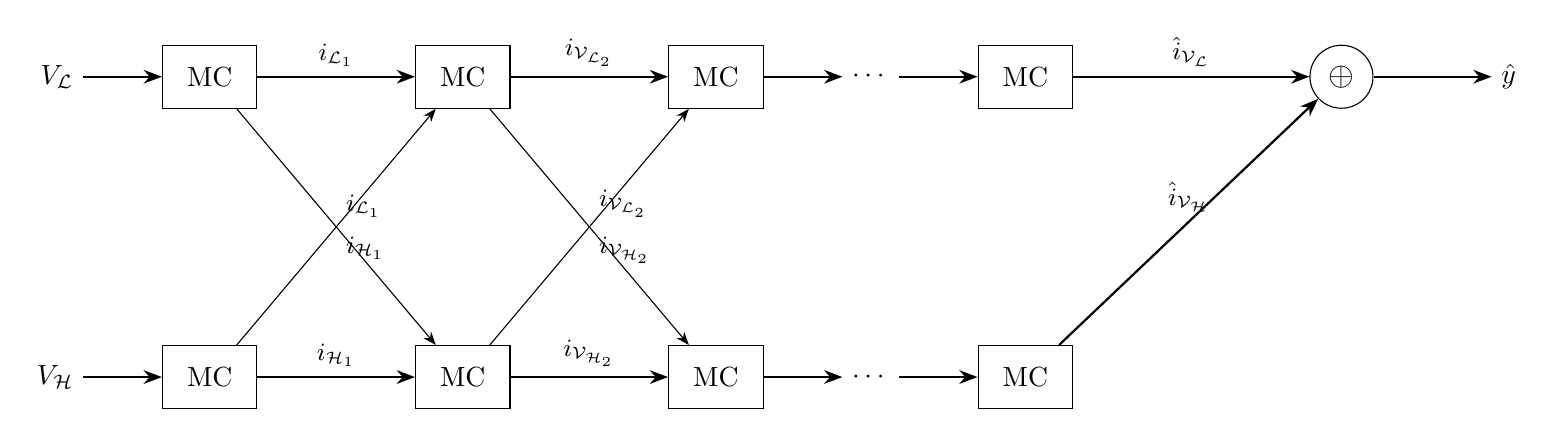
\begin{tikzpicture}[
    node distance=2.5cm and 2cm,
    >=Stealth,
    % 节点样式
    mc/.style={
        rectangle,
        draw=black,
        fill=white,
        minimum width=1.2cm,
        minimum height=0.8cm,
        font=\normalsize
    },
    sum/.style={
        circle,
        draw=black,
        fill=white,
        minimum size=0.8cm,
        font=\large
    },
    % 连接线样式
    main/.style={->, thick, black},
    cross/.style={->, black},
    label/.style={font=\small}
]

% 上层MC链
\node[mc] (mc1) {MC};
\node[mc, right=of mc1] (mc2) {MC};
\node[mc, right=of mc2] (mc3) {MC};
\node[right=1cm of mc3, font=\normalsize] (dots1) {$\cdots$};
\node[mc, right=1cm of dots1] (mc4) {MC};

% 下层MC链
\node[mc, below=3cm of mc1] (mc5) {MC};
\node[mc, right=of mc5] (mc6) {MC};
\node[mc, right=of mc6] (mc7) {MC};
\node[right=1cm of mc7, font=\normalsize] (dots2) {$\cdots$};
\node[mc, right=1cm of dots2] (mc8) {MC};

% 输入标签
\node[left=1cm of mc1] (vc) {$V_{\mathcal{L}}$};
\node[left=1cm of mc5] (vh) {$V_{\mathcal{H}}$};

% 求和节点
\node[sum, right=3cm of mc4] (sum1) {$\oplus$};

% 输出
\node[right=1.5cm of sum1] (output) {$\hat{y}$};

% 主连接线(上层)
\draw[main] (vc) -- (mc1);
\draw[main] (mc1) -- (mc2) node[midway, above, label] {$i_{\mathcal{L}_1}$};
\draw[main] (mc2) -- (mc3) node[midway, above, label] {$i_{\mathcal{V}_{\mathcal{L}_2}}$};
\draw[main] (mc3) -- (dots1);
\draw[main] (dots1) -- (mc4);

% 主连接线(下层)
\draw[main] (vh) -- (mc5);
\draw[main] (mc5) -- (mc6) node[midway, above, label] {$i_{\mathcal{H}_1}$};
\draw[main] (mc6) -- (mc7) node[midway, above, label] {$i_{\mathcal{V}_{\mathcal{H}_2}}$};
\draw[main] (mc7) -- (dots2);
\draw[main] (dots2) -- (mc8);

% 交叉连接
\draw[cross] (mc1) -- (mc6) node[midway, above right, label] {$i_{\mathcal{L}_1}$};
\draw[cross] (mc2) -- (mc7) node[midway, above right, label] {$i_{\mathcal{V}_{\mathcal{L}_2}}$};
\draw[cross] (mc5) -- (mc2) node[midway, below right, label] {$i_{\mathcal{H}_1}$};
\draw[cross] (mc6) -- (mc3) node[midway, below right, label] {$i_{\mathcal{V}_{\mathcal{H}_2}}$};

% 输出连接
\draw[main] (mc4) -- (sum1) node[midway, above, label] {$\hat{i}_{\mathcal{V}_{\mathcal{L}}}$};
\draw[main] (mc8) -- (sum1) node[midway, above, label] {$\hat{i}_{\mathcal{V}_{\mathcal{H}}}$};
\draw[main] (sum1) -- (output);

\end{tikzpicture}
\end{document}